%%%%%%%%%%%%%%%%%%%%%%%%%%%%%%%%%%%%%%%%%
% Beamer Presentation
% LaTeX Template
% Version 1.0 (10/11/12)
%
% This template has been downloaded from:
% http://www.LaTeXTemplates.com
%
% License:
% CC BY-NC-SA 3.0 (http://creativecommons.org/licenses/by-nc-sa/3.0/)
%
%%%%%%%%%%%%%%%%%%%%%%%%%%%%%%%%%%%%%%%%%

%----------------------------------------------------------------------------------------
%	PACKAGES AND THEMES
%----------------------------------------------------------------------------------------

\documentclass[t]{beamer}

\mode<presentation> {

% The Beamer class comes with a number of default slide themes
% which change the colors and layouts of slides. Below this is a list
% of all the themes, uncomment each in turn to see what they look like.

%\usetheme{default}
%\usetheme{AnnArbor}
%\usetheme{Antibes}
%\usetheme{Bergen}
%\usetheme{Berkeley}
%\usetheme{Berlin}
%\usetheme{Boadilla}
%\usetheme{CambridgeUS}
%\usetheme{Copenhagen}
%\usetheme{Darmstadt}
%\usetheme{Dresden}
%\usetheme{Frankfurt}
%\usetheme{Goettingen}
%\usetheme{Hannover}
%\usetheme{Ilmenau}
%\usetheme{JuanLesPins}
%\usetheme{Luebeck}
\usetheme{Madrid}
%\usetheme{Malmoe}
%\usetheme{Marburg}
%\usetheme{Montpellier}
%\usetheme{PaloAlto}
%\usetheme{Pittsburgh}
%\usetheme{Rochester}
%\usetheme{Singapore}
%\usetheme{Szeged}
%\usetheme{Warsaw}

% As well as themes, the Beamer class has a number of color themes
% for any slide theme. Uncomment each of these in turn to see how it
% changes the colors of your current slide theme.

%\usecolortheme{albatross}
%\usecolortheme{beaver}
%\usecolortheme{beetle}
%\usecolortheme{crane}
%\usecolortheme{dolphin}
%\usecolortheme{dove}
%\usecolortheme{fly}
%\usecolortheme{lily}
%\usecolortheme{orchid}
%\usecolortheme{rose}
%\usecolortheme{seagull}
%\usecolortheme{seahorse}
%\usecolortheme{whale}
%\usecolortheme{wolverine}

%\setbeamertemplate{footline} % To remove the footer line in all slides uncomment this line
%\setbeamertemplate{footline}[page number] % To replace the footer line in all slides with a simple slide count uncomment this line

%\setbeamertemplate{navigation symbols}{} % To remove the navigation symbols from the bottom of all slides uncomment this line
}
\usepackage[utf8]{vietnam}
\usepackage{amsmath}
\usepackage{graphicx} % Allows including images
\graphicspath{ {images/} }
%\usepackage{floatrow}
%\floatsetup[figure]{capposition=bottom}
\usepackage{caption}
\usepackage{booktabs} % Allows the use of \toprule, \midrule and \bottomrule in tables


%----------------------------------------------------------------------------------------
%	TITLE PAGE
%----------------------------------------------------------------------------------------

\title[Dự đoán xác suất xe buýt về trạm đúng giờ]{DỰ ĐOÁN XÁC SUẤT \\XE BUÝT VỀ TRẠM ĐÚNG GIỜ} % The short title appears at the bottom of every slide, the full title is only on the title page

\author[Lê Thị Minh Thùy]{Lê Thị Minh Thùy} % Your name
\institute[] % Your institution as it will appear on the bottom of every slide, may be shorthand to save space
{
Đại Học Bách Khoa TPHCM \\ % Your institution for the title page
\medskip
}
\date{\today} % Date, can be changed to a custom date

\begin{document}

\begin{frame}
\titlepage % Print the title page as the first slide
\end{frame}

\begin{frame}{Nội dung}
\begin{enumerate}
\item Giới thiệu đề tài
\item Dữ liệu
\item Phương pháp nghiên cứu
\item Cơ sở lý thuyết
\item Kết luận
\end{enumerate}
\end{frame}

%----------------------------------------------------------------------------------------
%	PRESENTATION SLIDES
%----------------------------------------------------------------------------------------
\begin{frame}[c]{ Giới thiệu đề tài}
\centering
Dự đoán xác suất xe buýt tuyến 72 \\ lộ trình xuất phát từ BX Củ Chi về trạm đích BX An Sương \\ đúng giờ (hạn mức 45 phút)
\end{frame}

%------------------------------------------------

\begin{frame}[t]
\frametitle{Dữ liệu thô}
Ví dụ 10 dữ liệu thô:\\
\begin{flushleft}
\begin{tabular}{ |l|l|l|l| }
\hline
&Vĩ độ & Kinh độ & Thời điểm xuất hiện \\ 
\hline
1&10.844095 & 106.613688333333 & 2016-09-02 07:25:43 \\ 
\hline
2&10.84298 & 106.614991666667 & 2016-09-02 07:26:02 \\
\hline
3&10.8424316666667 & 106.615195 & 2016-09-02 07:26:22 \\
\hline
4&10.8426816666667 & 106.615596666667 & 2016-09-02 07:26:42 \\
\hline
5&10.84309 & 106.615203333333 & 2016-09-02 07:27:02 \\
\hline
6&10.846395 & 106.61304 & 2016-09-02 07:30:48 \\
\hline
7&10.84664 & 106.612861666667 & 2016-09-02 07:31:01 \\
\hline
8&10.8475833333333 & 106.612253333333 & 2016-09-02 07:31:21 \\
\hline
9&10.8488916666667 & 106.611426666667 & 2016-09-02 07:31:41 \\
\hline
10&10.84932 & 106.61117 & 2016-09-02 07:31:53 \\
\hline 
\end{tabular}
\end{flushleft}
\end{frame}

%------------------------------------------------

\begin{frame}[t]
\frametitle{Dữ liệu làm việc}Dữ liệu sau khi được đồng bộ hóa khoảng cách thời gian hồi đáp (20 giây)\\
\begin{columns}[T] % align columns
\begin{column}{.3\textwidth}
\begin{tabular}{ |l|p{1cm}|p{1cm}| }
\hline
STT&Khoảng cách thời gian hồi đáp (giây) & Khoảng cách bước đi (mét)\\
\hline
\hline
1&20&71\\
\hline
2&20& 86\\
\hline
3&20& 145\\
\hline
4&20& 136\\
\hline
5&20& 104\\
\hline
6&20& 277\\
\hline
7&20& 240\\
\hline
8&20& 145\\
\hline
9&20& 97\\
\hline
\end{tabular}
\end{column}%
\hfill%
\begin{column}{.3\textwidth}
\begin{tabular}{ |l|p{1cm}|p{1cm}| }
\hline
STT&Khoảng cách thời gian hồi đáp (giây) & Khoảng cách bước đi (mét)\\
\hline
\hline
10&20& 0\\
\hline
11&20& 171\\
\hline
12&20& 283\\
\hline
13&20& 283\\
\hline
14&20& 0\\
\hline
15&20& 214\\
\hline
16&20& 166\\
\hline
17&20& 307\\
\hline
18&20& 259\\
\hline
\end{tabular}
\end{column}%
\hfill%
\begin{column}{.3\textwidth}
\begin{tabular}{ |l|p{1cm}|p{1cm}| }
\hline
STT&Khoảng cách thời gian hồi đáp (giây) & Khoảng cách bước đi (mét)\\
\hline
\hline
85&20& 132\\
\hline
86&20& 52\\
\hline
87&20& 44\\
\hline
88&20& 63\\
\hline
89&20& 63\\
\hline
90&20& 46\\
\hline
91&20& 46\\
\hline
92&21& 40\\
\hline
93&17& 236\\
\hline
\end{tabular}
\end{column}%
\end{columns}
\end{frame}

%------------------------------------------------

\begin{frame}[t]
\frametitle{Dữ liệu trực quan hóa}Trực quan hóa giá trị các bước di chuyển trong 80\% thời gian di chuyển\\
\begin{center}
\begin{minipage}{0.48\linewidth}
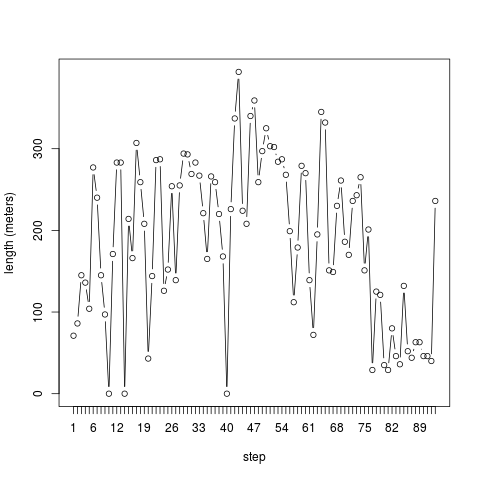
\includegraphics[width=\linewidth]{test_80_1}
\captionof*{figure}{Chuyến xe 1 - đúng giờ}
\end{minipage}%
\hfill
\begin{minipage}{0.49\linewidth}
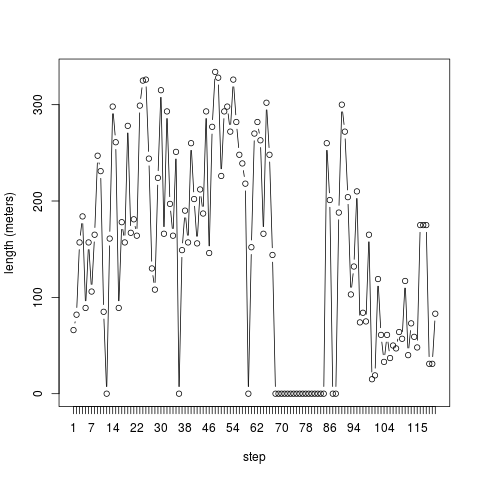
\includegraphics[width=\linewidth]{test_80_2}
\captionof*{figure}{Chuyến xe 2 - trễ giờ}
\end{minipage}
\end{center}
\end{frame}

%------------------------------------------------

\begin{frame}
\frametitle{Phương pháp nghiên cứu}
\begin{itemize}
\item số lượng dữ liệu mẫu giới hạn
\item các bước di chuyển cách nhau 20 giây
\item 80\% lộ trình từ BX Củ Chi - BX An Sương
\item trực quan hóa dữ liệu
\item nếu có nhiều bước di chuyển dài thì xác suất về trạm đúng giờ cao
\item chấp nhận có yếu tố ngẫu nhiên ảnh hưởng đến kết quả dự đoán 
\end{itemize}
\end{frame}

%------------------------------------------------

\begin{frame}[t]
\frametitle{Cơ sở lý thuyết}
\begin{minipage}{0.48\linewidth}
\begin{itemize}
\item Thống Kê
\item Không gian mẫu và biến cố
\item Xác suất của biến cố
\item Xác suất có điều kiện và sự độc lập của các biến cố
\item Biến ngẫu nhiên
\item Biến ngẫu nhiên rời rạc
\item Biến ngẫu nhiên liên tục
\end{itemize}
\end{minipage}%
\hfill
\begin{minipage}{0.49\linewidth}
\begin{itemize}
\item Xác suất Bayes
\item Vấn đề thực tế khi áp dụng xác suất Bayes
\item Phân phối chuẩn Gauss
\item Phân loại Gaussian Bayes
\item Thuật toán Kernel Density Estimation 
\end{itemize}
\end{minipage}
\end{frame}

%------------------------------------------------

\begin{frame}
\frametitle{Cơ sở lý thuyết - Thống Kê}
\begin{block}{Unofficial definition of statistics}
Statistics is the science of problem-solving in the presence of \textbf{\underline{variability}}.
\end{block}
Explain the word "variability"\footnote{http://www.stat.uci.edu/what-is-statistics/}:
\begin{itemize}
\item There are many situations that we encounter in science (or more generally in life) in which the outcome is uncertain.
\item If the same measurement were repeated, then the answer would likely change
\end{itemize}
\end{frame}

%------------------------------------------------

\begin{frame}
\frametitle{Cơ sở lý thuyết - Không gian mẫu và biến cố}
\begin{block}{Định nghĩa không gian mẫu}
Không gian mẫu là tập hợp của tất cả các kết cục có thể của một thí nghiệm cụ thể.
\end{block}
\begin{block}{Định nghĩa biến cố}
Các biến cố sơ cấp hay điểm mẫu là những phần tử của không gian mẫu.
\end{block}
\underline{Ví dụ}:\\ 
Thí nghiệm tung một đồng xu, kết quả ngẫu nhiên là ngửa (Head, $\mathcal{H}$) hoặc sấp (Tail, $\mathcal{T}$), cho ta không gian mẫu $\mathcal{S= \{H,T}\}$\\
Các biến cố sơ cấp hay điểm mẫu là những phần tử của $\mathcal{S}$

\end{frame}


%------------------------------------------------

\begin{frame}[t]
\frametitle{Cơ sở lý thuyết - Xác suất của biến cố}
Tập các biến cố $\mathcal{Q}$ := $\{ A: A \subset \mathcal{S}$ là một biến cố$\}$\\
Xét một hàm $\mathbb{P}: \mathcal{Q} \rightarrow \mathbb{R}$\\
$\mathbb{P}$(A) là khả năng hoặc cơ hội mà biến cố A xảy ra.\\
$\mathbb{P}$ được gọi là hàm xác suất khi thỏa mãn những tiên đề cơ bản sau đây:\\
\begin{itemize}
\item $\mathbb{P}$(A) $\geq$ 0
\item $\mathbb{P}(\mathcal{S})$=1
\item Nếu ta có $E_{1}, E_{2},...,E_{n}$ (n $\geq$ 1) là các biến cố rời nhau từng đôi một thì\\
\[
\mathbb{P}\left[\bigcup_{i=1}^n E_{i}\right]=\sum_{i=1}^n \mathbb{P}[E_i]
\]
\end{itemize}
\end{frame}

%------------------------------------------------

\begin{frame}[t]
\frametitle{Cơ sở lý thuyết - Xác suất có điều kiện và sự độc lập của các biến cố}
Nếu biến cố A xảy ra phụ thuộc vào biến cố B đã xảy ra $\mathbb{P}[B]$ > 0 thì xác suất đồng thời của hai biến cố A và B:
\[
\mathbb{P}(AB)=\mathbb{P}(A\cap B)=\mathbb{P}(B)\cdot \mathbb{P}(A|B)
\]
Nếu biến cố A và B độc lập, sự xuất hiện của A không có liên quan đến sự xuất hiện của B thì xác suất đồng thời của hai biến cố A và B:
\[
\mathbb{P}(AB)=\mathbb{P}(A\cap B)=\mathbb{P}(A)\cdot\mathbb{P}(B)
\]
\end{frame}

%------------------------------------------------

\begin{frame}[t]
\frametitle{Cơ sở lý thuyết - Biến ngẫu nhiên}
\begin{block}{Định nghĩa biến ngẫu nhiên}
Một biến ngẫu nhiên là một hàm giá trị thực $X(\omega)$ (hay X) xác định trên một không gian mẫu $\mathcal{S}$, sao cho các biến cố $\{\omega \in \mathcal{S}: X(\omega) \leq x\}$ có thể được gán các xác suất, với mọi  $-\infty < x < \infty$. Ta ghi $X: \mathcal{S} \rightarrow \mathbb{R}$. Thật vậy, với bất kỳ $x \in \mathbb{R}$, tập tiền ảnh $\{\omega \in \mathcal{S}:X(\omega) \leq x\}\subseteq \mathcal{S}$ rõ ràng là một biến cố, và được ký hiệu là A = X $\leq$ x hay $\{X \leq x\}$. Vậy xác suất $\mathbb{P}[A]$=$\mathbb{P}[X \leq x]$ luôn tồn tại.
\end{block}
\end{frame}

%------------------------------------------------

\begin{frame}[t]
\frametitle{Cơ sở lý thuyết - Biến ngẫu nhiên rời rạc}
\begin{block}{Định nghĩa biến ngẫu nhiên rời rạc}
X(.) là biến có một phạm vi $\mathcal{S}_X = X(\mathcal{S})$ là tập giá trị rời rạc (hữu hạn hoặc vô hạn đếm được, nghĩa là có lượng số không quá lượng số tập tự nhiên $\mathbb{N}$)
\end{block}
\textbf{Bảng phân phối xác suất} của X được cho bởi\\
\begin{center}
\begin{tabular}{ rccccc }
\specialrule{.1em}{.05em}{.05em} 
X & $x_0$ & $x_1$ & ... & $x_{m-1}$ & $x_{m}$\\
\hline
p$_k$:=$p(x_k$)=$\mathbb{P}$[X=$x_k$] & $p_0$ & $p_1$ & ... & $p_{m-1}$ & $p_m$\\
\specialrule{.1em}{.05em}{.05em} 
\end{tabular}
\end{center}
\end{frame}

%------------------------------------------------

\begin{frame}[t]
\frametitle{Cơ sở lý thuyết - Biến ngẫu nhiên rời rạc}
\textbf{Tập giá trị} 
\[
\mathcal{S}_X = \{x_0, x_1, x_2, ..., x_{m-1}, x_m\}, m \in \mathbb{N}
\]
\textbf{Hàm mật độ xác suất}\\
\[
p(x) = \mathbb{P}[X=x]= \mathbb{P}[\{\omega: X(\omega)=x\}], x \in \mathcal{S}_X
\]
với $p(x) \geq 0$ và $\sum_{x \in \mathcal{S}_X} p(x) = 1$\\
\textbf{Hàm tích lũy xác suất}
\[
F_{X}(x) = \mathbb{P}[X\leq x] = \mathbb{P}[{\omega \in S: X(\omega) \leq x}]=\sum_{x_k\leq x} p(x_k)
 = \sum_{x_k\leq x} p_k,   x \in \mathbb{R}
\] 
\textbf{Kỳ vọng} (hay trung bình)
\[
\mu = \mathbb{E}[X] = \sum_{x_k \in \mathcal{S}_X} x_k p_k
\]
\textbf{Phương sai}
\[
\sigma^2 = \mathbb{E}[(X-\mu)^2] = \sum_{x_k \in \mathcal{S}_X} [x_k - \mu]^2 p_k
\]
\textbf{Độ lệch chuẩn} $\sigma_{X} = \sigma = \sqrt{Var(X)}$
\end{frame}

%------------------------------------------------

\begin{frame}[t]
\frametitle{Cơ sở lý thuyết - Biến ngẫu nhiên liên tục}
\begin{block}{Định nghĩa biến ngẫu nhiên liên tục}
X(.) là liên tục khi nó có phạm vi bao gồm khoảng con (hay toàn bộ) tập số thực, nghĩa là $\mathcal{S}_X \in \mathbb{R}$
\end{block}
\textbf{Tập giá trị} X nhận vô hạn giá trị không đếm được, $\mathcal{S}_X \subset \mathbb{R}$\\
\textbf{Hàm mật độ xác suất}\\
Tính chất của hàm mật độ xác suất f gồm:
\begin{itemize}
\item f(u) $\geq$ 0, $\forall$u.
\item $\int_{-\infty}^{\infty} f(u)du$ = 1 = F($-\infty$)
\item 
\[
\mathbb{P}(a \leq X \leq b) = \mathbb{P}(a < X < b) = \mathbb{P}(a \leq X < b)
\]
\[
 = \int_{a}^{b} f(u)du = F(b) - F(a)
\]
\item Đạo hàm $f(x) = \frac{dF(x)}{dx}$ có thể không tồn tại ở một số hữu hạn giá trị x, trong khoảng hữu hạn bất kỳ.   
\end{itemize}
\end{frame}

%------------------------------------------------

\begin{frame}[t]
\frametitle{Cơ sở lý thuyết - Biến ngẫu nhiên liên tục}
\textbf{Hàm tích lũy xác suất}\\
Tồn tại một hàm số không âm $f(u)$ thỏa
\[
F(x) = \mathbb{P}(X \leq x) = \int_{-\infty}^{x} f(u)d(u), \infty < x < -\infty 
\]
F(x) gọi là hàm phân phối (tích lũy) xác suất (c.d.f) của X, f(u) là hàm mật độ của X\\
Tính chất của hàm phân phối xác suất F gồm:
\begin{itemize}
\item F liên tục, và
\item $\lim_{x->-\infty}$ F(x)=0, $\lim_{x->\infty}$F(x)=1
\item F không giảm, nghĩa là nếu $x_1$ < $x_2$ thì F($x_1$) $\leq$ F($x_2$), và
\item Quan hệ với f: hàm phân phối xác suất F(x) có đạo hàm $\frac{dF(x)}{dx}$ = f(x)     
\end{itemize}
\end{frame}

%------------------------------------------------

\begin{frame}[t]
\frametitle{Cơ sở lý thuyết - Xác suất Bayes}
\begin{block}{Định nghĩa}
Bayes’ theorem describes the probability of an event, based on prior knowledge of conditions that might be related to the event.\\
\center
$\mathbb{P}(B|A) = \frac{\mathbb{P}(B) \cdot \mathbb{P}(A|B)}{\mathbb{P}(A)}$
\end{block}
\end{frame}

%------------------------------------------------

\begin{frame}[t]
\frametitle{Cơ sở lý thuyết - Vấn đề thực tế khi áp dụng xác suất Bayes}
Biến hoặc giá trị biến rtrên thực tế \underline{rất hiếm khi được phân loại}, trong khi giải thuật xác suất Bayes $\mathbb{P}(B|A) = \frac{\mathbb{P}(B) \cdot \mathbb{P}(A|B)}{\mathbb{P}(A)}$ làm việc với biến và giá trị biến được phân loại.\\
Trong Luận Văn này:
\begin{itemize}
\item Biến là những bước di chuyển
\item Giá trị biến là số lần lặp lại những bước di chuyển đó
\end{itemize}
\end{frame}


%------------------------------------------------

\begin{frame}[t]
\frametitle{Cơ sở lý thuyết - Vấn đề thực tế khi áp dụng xác suất Bayes}
Có hai hướng giải quyết đối với thuộc tính ở dạng con số
\begin{itemize}
\item Rời rạc hóa thuộc tính dạng con số thành dạng phân loại => Dễ tranh cãi
\item Sử dụng hàm mật độ xác suất cho biến liên tục
\end{itemize}
\end{frame}

%------------------------------------------------

\begin{frame}[t]
\frametitle{Cơ sở lý thuyết - Phân phối chuẩn (Gauss)}
Biến ngẫu nhiên $\mathit{X}$ có hàm mật độ là hàm
\[
f(x)=n(x,\mu,\sigma)=\frac{1}{\sigma\sqrt{2\pi}} * e^{-\frac{(x-\mu)^2}{2\sigma^2}} -\infty < x < \infty, \mu \in \mathbb{R}, \sigma^2 > 0
\]
Ký hiệu $\mathit{X} \thicksim \textbf{N}(\mu,\sigma)$\\
\end{frame}

%------------------------------------------------

\begin{frame}[t]
\frametitle{Cơ sở lý thuyết - Phân phối chuẩn (Gauss)}
\begin{figure}[h]
  \centering
    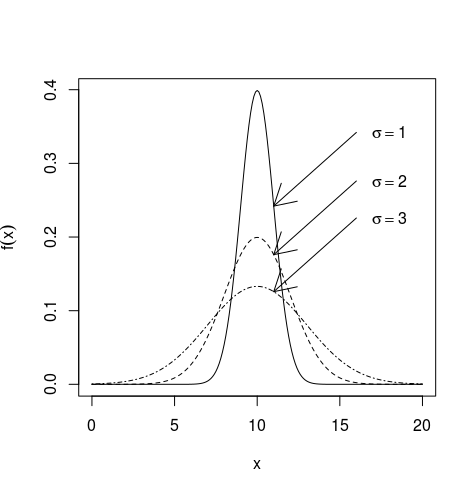
\includegraphics[width=0.5\textwidth]{Normal_Distribution_PDF.png}   
    \caption*{Hàm mật độ của $\textbf{N}(\mu,\sigma)$ với $\mu=10, \sigma=1,2,3$} 
\end{figure}
\end{frame}

%------------------------------------------------

\begin{frame}[t]
\frametitle{Cơ sở lý thuyết -- Phân loại Gaussian Bayes}
Gọi X là biến đầu vào\\
Gọi Y là biến phân loại lớp 0 hoặc 1, có xác suất $\mathrm{P_Y}(0)$=$\mathrm{P_Y}(1)$=$\frac{1}{2}$\\
Công thức hàm phân phối Gaussian 
$
\mathrm{G}(x,\mu,\sigma)=\frac{1}{\sqrt{2\pi\sigma^2}} * e^{-\frac{(x-\mu)^2}{2\sigma^2}}  
$\\
với $\mu=\frac{\sum_1^n x_i}{n}$ và $\sigma^2=\frac{\sum_1^n (x_i-\mu)^2}{n}$\\
Biến X có hàm phân phối Gaussian khác nhau theo mỗi phân loại, nghĩa là \\
$\mathrm{P_{X|Y}}(x|0)=\mathrm{G}(x,\mu_0,\sigma_0)$\\
$\mathrm{P_{X|Y}}(x|1)=\mathrm{G}(x,\mu_1,\sigma_1)$\\
\begin{figure}[h]
  \centering
    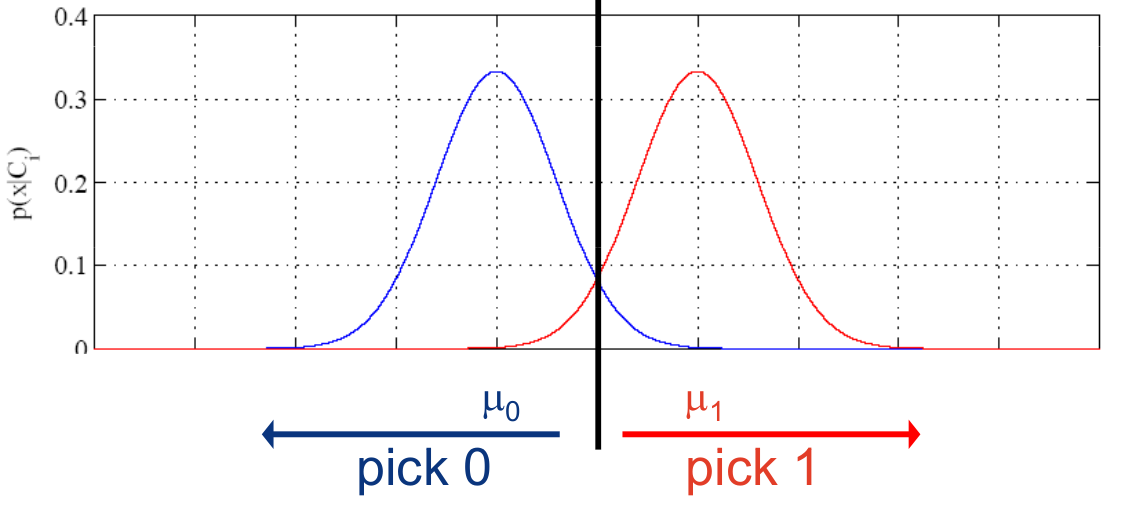
\includegraphics[width=0.5\textwidth]{GaussBayesEx2.png}    
\end{figure}
Nếu x < $\frac{\mu_1+\mu_2}{2}$ thì phân loại x vào 0, nếu x > $\frac{\mu_1+\mu_2}{2}$ thì phân loại x vào 1.
\end{frame}

%------------------------------------------------

\begin{frame}[t]
\frametitle{Cơ sở lý thuyết -- Thuật toán Kernel Density Estimation\footnote{https://chemicalstatistician.wordpress.com/2013/06/09/exploratory-data-analysis-kernel-density-estimation-in-r-on-ozone-pollution-data-in-new-york-and-ozonopolis/}}
\begin{block}{What is Kernel Density Estimation?}
In statistics, \underline{kernel} density estimation (KDE) is \underline{a non-parametric way} to estimate \underline{the probability density function} of a continuous random variable based on a finite data sample.
\end{block}
\begin{itemize}
\item A kernel is a special type of probability density function (PDF) with the added property that it must be even. 
\item Non-parametric models differ from parametric models in that the model structure is not specified a priori but is instead determined from data. The term non-parametric is not meant to imply that such models completely lack parameters but that the number and nature of the parameters are flexible and not fixed in advance.
\end{itemize}
\end{frame}

%------------------------------------------------

\begin{frame}[t]
\frametitle{Cơ sở lý thuyết -- Thuật toán Kernel Density Estimation}
Constructing a Kernel Density Estimate: Step by Step
\begin{enumerate}
\item Choose a kernel, the common ones are normal (Gaussian), uniform (rectangular) and triangular.
\item At each datum, $x_i$, build the scaled kernel function\\
$K_h = \frac{1}{h}K[\frac{(x-x_1)}{h}]$\\
where $K()$ is your chosen kernel function. The paramter $h$ is called the bandwidth, the window width, or the smoothing paramter.
\item Add all of the individual scaled kernel functions and divide by $n$; this places a probability of $\frac{1}{n}$ to each $x_i$. It also ensures that the kernel density estimate integrates to 1 over its support set.\\
\[
\hat{f}(x_i) = \hat{p}_{KDE}(x_i) = \frac{1}{n}\sum_{i=1}^{n} K_h = \frac{1}{n}\frac{1}{h}\sum_{i=1}^{n} K(\frac{x-x_i}{h})
\]
\end{enumerate}
\end{frame}

%------------------------------------------------

\begin{frame}
\frametitle{Cơ sở lý thuyết -- Thuật toán Kernel Density Estimation\footnote{https://en.wikipedia.org/wiki/Kernel\_density\_estimation}}
Thuật toán Kernel Density Estimation
\begin{center}
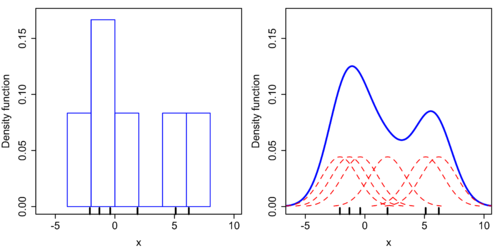
\includegraphics[height=2in,width=3in]{500px-Comparison_of_1D_histogram_and_KDE.png}
\end{center}
\end{frame}

%------------------------------------------------

\begin{frame}
\frametitle{Cơ sở lý thuyết -- Thuật toán Kernel Density Estimation}
Choosing the Bandwidth\\
It turns out that the choosing the bandwidth is the most difficult step in creating a good kernel density estiamte that captures the underlying distribution of the variable.\\
\end{frame}

%------------------------------------------------

\begin{frame}
\frametitle{Cơ sở lý thuyết -- Thuật toán Kernel Density Estimation}
Thuật toán Kernel Density Estimation
\begin{center}
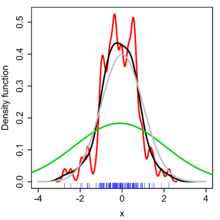
\includegraphics[height=2in,width=3in]{220px-Comparison_of_1D_bandwidth_selectors.png}
\end{center}
\end{frame}

%------------------------------------------------

\begin{frame}
\frametitle{Kết Luận}
\begin{block}{Bài toán}
Dự đoán xác suất xe buýt tuyến 72 lộ trình xuất phát từ BX Củ Chi về trạm đích BX An Sương đúng giờ (hạn mức 45 phút)
\end{block}
Dữ liệu thô là tọa độ vĩ độ, kinh độ và thời điểm xuất hiện tại vị trí đó của xe buýt\\
Ví dụ 7 dữ liệu thô:\\
\begin{flushleft}
\begin{tabular}{ |l|l|l|l| }
\hline
&Vĩ độ & Kinh độ & Thời điểm xuất hiện \\ 
\hline
1&10.844095 & 106.613688333333 & 2016-09-02 07:25:43 \\ 
\hline
2&10.84298 & 106.614991666667 & 2016-09-02 07:26:02 \\
\hline
3&10.8424316666667 & 106.615195 & 2016-09-02 07:26:22 \\
\hline
4&10.8426816666667 & 106.615596666667 & 2016-09-02 07:26:42 \\
\hline
5&10.84309 & 106.615203333333 & 2016-09-02 07:27:02 \\
\hline
6&10.846395 & 106.61304 & 2016-09-02 07:30:48 \\
\hline
7&10.84664 & 106.612861666667 & 2016-09-02 07:31:01 \\
\hline 
\end{tabular}
\end{flushleft}
\end{frame}

%------------------------------------------------

\begin{frame}[t]
\frametitle{Kết Luận}Chỉ giữ lại các bước di chuyển trong 80\% thời gian đầu\\
\begin{center}
\begin{minipage}{0.48\linewidth}
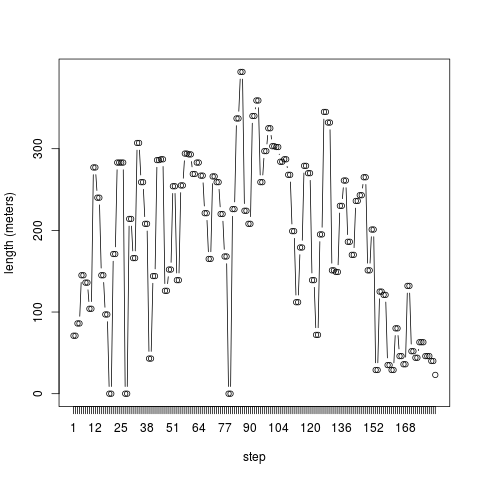
\includegraphics[width=\linewidth]{test1}
\captionof*{figure}{Toàn bộ di chuyển chuyến xe 1}
\end{minipage}%
\hfill
\begin{minipage}{0.49\linewidth}
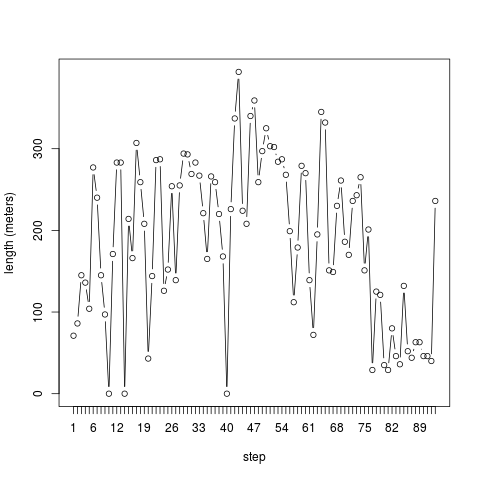
\includegraphics[width=\linewidth]{test_80_1}
\captionof*{figure}{80\% di chuyển chuyến xe 1}
\end{minipage}
\end{center}
\end{frame}

%------------------------------------------------

\begin{frame}
\frametitle{Kết Luận}
Dữ liệu làm việc là dữ liệu sau khi được đồng bộ hóa khoảng cách thời gian hồi đáp (20 giây)\\
\begin{columns}[T] % align columns
\begin{column}{.3\textwidth}
\begin{tabular}{ |l|p{1cm}|p{1cm}| }
\hline
STT&Khoảng cách thời gian hồi đáp (giây) & Khoảng cách bước đi (mét)\\
\hline
\hline
1&20&71\\
\hline
2&20& 86\\
\hline
3&20& 145\\
\hline
4&20& 136\\
\hline
5&20& 104\\
\hline
6&20& 277\\
\hline
7&20& 240\\
\hline
8&20& 145\\
\hline
9&20& 97\\
\hline
\end{tabular}
\end{column}%
\hfill%
\begin{column}{.3\textwidth}
\begin{tabular}{ |l|p{1cm}|p{1cm}| }
\hline
STT&Khoảng cách thời gian hồi đáp (giây) & Khoảng cách bước đi (mét)\\
\hline
\hline
10&20& 0\\
\hline
11&20& 171\\
\hline
12&20& 283\\
\hline
13&20& 283\\
\hline
14&20& 0\\
\hline
15&20& 214\\
\hline
16&20& 166\\
\hline
17&20& 307\\
\hline
18&20& 259\\
\hline
\end{tabular}
\end{column}%
\hfill%
\begin{column}{.3\textwidth}
\begin{tabular}{ |l|p{1cm}|p{1cm}| }
\hline
STT&Khoảng cách thời gian hồi đáp (giây) & Khoảng cách bước đi (mét)\\
\hline
\hline
85&20& 132\\
\hline
86&20& 52\\
\hline
87&20& 44\\
\hline
88&20& 63\\
\hline
89&20& 63\\
\hline
90&20& 46\\
\hline
91&20& 46\\
\hline
92&21& 40\\
\hline
93&17& 236\\
\hline
\end{tabular}
\end{column}%
\end{columns}
\end{frame}

%------------------------------------------------

\begin{frame}
\frametitle{Kết Luận}
Bài toán này sẽ có 5 biến: 
\begin{itemize}
\item $X_1$: bước di chuyển 0-15 km/h
\item $X_2$: bước di chuyển 15-30 km/h
\item $X_3$: bước di chuyển 30-45 km/h
\item $X_4$: bước di chuyển 45-60 km/h
\item $X_5$: bước di chuyển 60 km/h
\end{itemize}
\end{frame}

%------------------------------------------------

\begin{frame}
\frametitle{Kết Luận}
Ta chọn thời gian hoàn thành trước đúng 45 phút là về đích đúng giờ\\
Như vậy ta có $\mathrm{P}$(về đích đúng giờ) = 0.84 và $\mathrm{P}$(về đích trễ giờ) = 0.16
\begin{center}
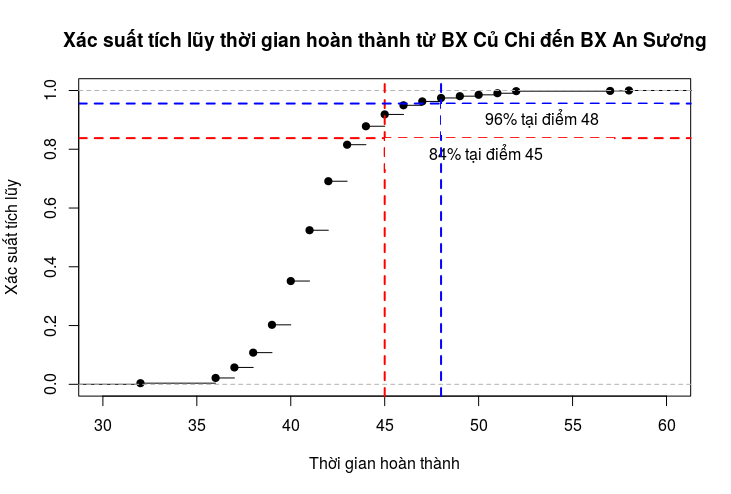
\includegraphics[height=2in,width=3in]{finishTime_CC_AS_ACC_Line}
\end{center}
\end{frame}

%------------------------------------------------
\begin{frame}
\frametitle{Kết Luận}
Dùng giải thuật Kernel Density Estimation để vẽ hàm mật độ xác suất của các biến dưới đây:\\
Hàm mật độ xác suất của biến $X_1$ bước đi 0-15 km/h
\begin{center}
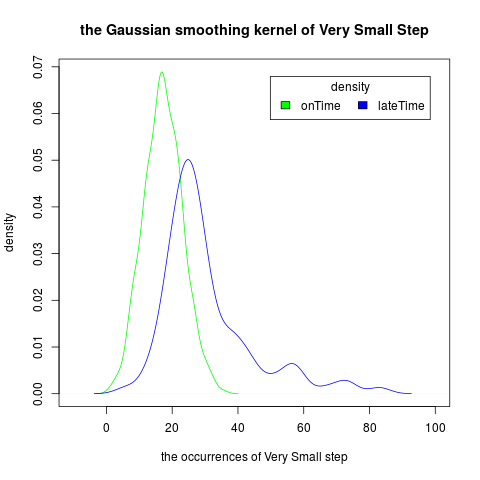
\includegraphics[height=2.7in,width=4in]{DensityVerySmallStep.png}
\end{center}
\end{frame}

%------------------------------------------------

\begin{frame}
\frametitle{Kết Luận}
Hàm mật độ xác suất của biến $X_2$ bước đi 15-30 km/h
\begin{center}
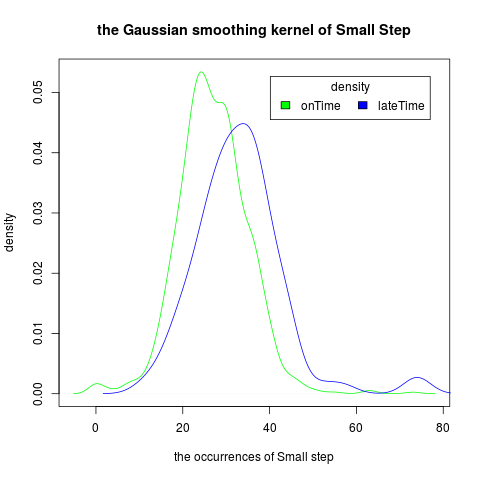
\includegraphics[height=2.7in,width=4in]{DensitySmallStep.png}
\end{center}
\end{frame}

%------------------------------------------------

\begin{frame}
\frametitle{Kết Luận}
Hàm mật độ xác suất của biến $X_3$ bước đi 30-45 km/h
\begin{center}
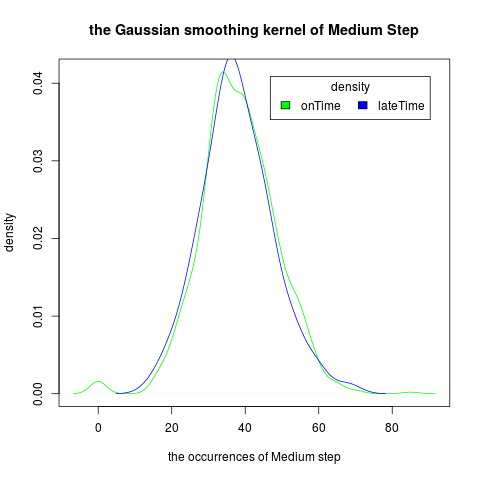
\includegraphics[height=2.7in,width=4in]{DensityMediumStep.png}
\end{center}
\end{frame}

%------------------------------------------------

\begin{frame}
\frametitle{Kết Luận}
Hàm mật độ xác suất của biến $X_4$ bước đi 45-60 km/h
\begin{center}
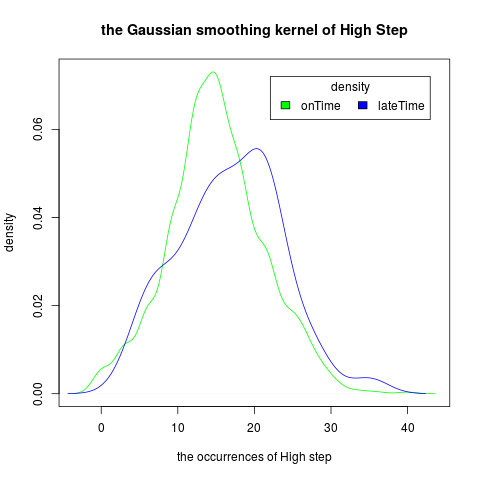
\includegraphics[height=2.7in,width=4in]{DensityHighStep.png}
\end{center}
\end{frame}

%------------------------------------------------
\begin{frame}
\frametitle{Kết Luận}
Hàm mật độ xác suất của biến $X_5$ trên 60 km/h
\begin{center}
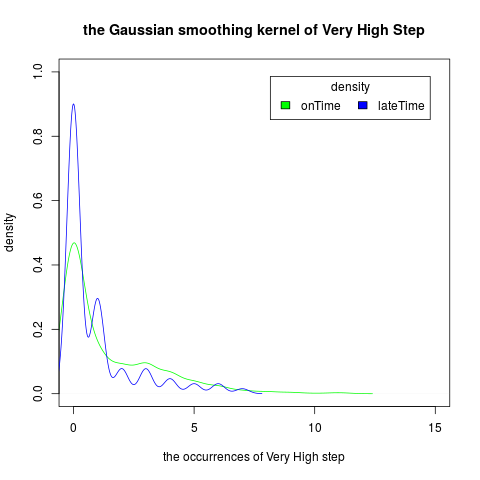
\includegraphics[height=2.7in,width=4in]{DensityVeryHighStep.png}
\end{center}
\end{frame}

%------------------------------------------------
\begin{frame}
\frametitle{Kết Luận}
Tìm xác suất của điểm mới\\
Nếu sử dụng nhân Gaussian trong thuật toán Kernel Density Estimation, ta có công thức tính xác suất của điểm mới
\[
\hat{f}(x_i) = \hat{p}_{KDE}(x_i) = \frac{1}{n}\sum_{i=1}^{n} K_h = \frac{1}{n}\frac{1}{h}\sum_{i=1}^{n} K(\frac{x-x_i}{h})
\]
\end{frame}

%------------------------------------------------
\begin{frame}
\frametitle{Kết luận}
Áp dụng Gaussian Bayes để dự đoán xác suất xe buýt về trạm đúng giờ\\
Cho dữ liệu kiểm tra $x$ có giá trị $x_1$, $x_2$, $x_3$, $x_4$, $x_5$\\
\[
\mathrm{P}(onTime|x) = \frac{\mathrm{P}(x|onTime)\mathrm{P}(onTime)}{\mathrm{P}(x|onTime)\mathrm{P}(onTime)+\mathrm{P}(x|lateTime)\mathrm{P}(lateTime)}
\]
Ta có $\mathrm{P}(onTime)$ = 0.84 và $\mathrm{P}(lateTime)$ = 0.16\\
Do các biến cố $X_1, X_2, X_3, X_4, X_5$ là các biến cố độc lập lẫn nhau cho nên\\
nghĩa là $\mathrm{P}(x|onTime) = \mathrm{P}(x_1|onTime)\mathrm{P}(x_2|onTime)\mathrm{P}(x_3|onTime)\mathrm{P}(x_4|onTime)\mathrm{P}(x_5|onTime)$ \\
và $\mathrm{P}(x|lateTime) = \mathrm{P}(x_1|lateTime)\mathrm{P}(x_2|lateTime)\mathrm{P}(x_3|lateTime)\mathrm{P}(x_4|lateTime)\mathrm{P}(x_5|lateTime)$
\end{frame}
%------------------------------------------------
%------------------------------------------------
\begin{frame}
\frametitle{Danh mục các tài liệu kham khảo}
\begin{thebibliography}{}
\bibitem{timeDependentGraph} Người dịch: Nguyễn Văn Minh Mẫn \emph{Thống kê Công nghiệp hiện đại với ứng dụng viết trên R, MINITAB và JMP}. Nhà xuất bản Bách Khoa Hà Nội,2016.
\bibitem{Gaussian classifier}
	\emph{Naive Bayes 3: Gaussian example}, truy cập ngày 2 tháng 3 năm 2017,
	địa chỉ \emph{https://www.youtube.com/watch?v=r1in0YNetG8}.	
\bibitem{DKE2}
	\emph{Exploratory Data Analysis: Kernel Density Estimation in R on Ozone Pollution Data in New York and Ozonopolis}, truy cập ngày 26 tháng 3 năm 2017,
	địa chỉ \emph{https://www.r-bloggers.com/exploratory-data-analysis-kernel-density-estimation-in-r-on-ozone-pollution-data-in-new-york-and-ozonopolis/}.
\end{thebibliography}
\end{frame}

%------------------------------------------------
\begin{frame}[c]{ }
\begin{Huge}
\centering
Thank you\\Q\&A\\
\end{Huge}
\end{frame}
%------------------------------------------------
\end{document} 